\documentclass[10pt,
%superscriptaddress,
%groupedaddress,
%unsortedaddress,
%runinaddress,
%frontmatterverbose, 
%preprint,
%preprintnumbers,
%nofootinbib,
%nobibnotes,
%bibnotes,
 amsmath,amssymb,
 aps,prb, twocolumn
]{revtex4-2}

% Graphics and math
\usepackage{empheq}
\usepackage{graphicx}
\usepackage{bm}
\usepackage{dcolumn}
\usepackage{physics}
\usepackage{soul}
\usepackage{dsfont}
\usepackage{xcolor} % for more colors
\usepackage[percent]{overpic} % for captions
% Subfigures (compatible with REVTeX)
\usepackage[caption=false]{subfig}  
%\captionsetup[subfloat]{position=top,justification=raggedright,singlelinecheck=false}
% Hyperlinks (must come last)
\usepackage[colorlinks=true,allcolors=blue]{hyperref}


\newcommand{\id}{\mathds{1}}
\newcommand\sj[1]{ {\color{cyan} #1} } 
\newcommand\jm[1]{ {\color{magenta} #1} } 
\definecolor{mediumgreen}{HTML}{228B22} % forest green-ish
\newcommand\oz[1]{ {\color{mediumgreen} #1} } 


\begin{document}


\title{Reflectometry Beyond Weak Measurement}

\author{Santiago Salazar Jaramillo}
\email{santiago.salazar-jaramillo@uni-konstanz.de}

\author{Jeff Maki}
% \email{jeffrey.maki@uni-konstanz.de}

\author{Oded Zilberberg}
% \email{oded.zilberberg@uni-konstanz.de}

\affiliation{Department of Physics, University of Konstanz, 78464 Konstanz, Germany}

\date{\today}

\begin{abstract}
    We develop a minimal model of a single measurement event between a qubit and a detector particle...
\end{abstract}

\maketitle

\section{Introduction}\label{sect:intro}
\begin{itemize}

     \item The study of weak (non-invasive) measurements has resulted in novel phenomena like continuous measurement \cite{wisemanQuantumTrajectorie1996,bauerRepeatedNonDemolition2013}, weak values \cite{aharonov1988, alonso2005, zilberbergSensingAmplification2011, romito2012} and the quantum Zeno effect \cite{doggenzeno2023}. 
    
     \item Von Neumann's indirect measurement scheme \cite{vonNeumann1932} realizes them by considering that system and detector are unitarily entangled during a finite time window by the interaction potential, which is assumed to fulfill non-demolition, afterwards readout is performed by projecting the detector, thus inducing a non-unitary jump and leaving the qubit in a new superposition of states. \cite{tamir013}.
    
    \item Nowadays modern detectors are capable of realizing von Neuman's weak measurement scheme \cite{field1993,pilgramEfficiencyMesoscopic2002, boissonneaultDispersiveNondemo2009}, among them QPC's are widely employed for charge readout of quantum dots \cite{reillyFastSinglechargeSensing2007, peterssonOneElectron2010, vandersypenDetectionElectron2004}, \sj{although maximizing the non-demolition aspect remains a technical challenge, impacting readout} \cite{kumbhakarShotNoise2025, boissonneaultDispersiveCircuit2009}.
    
    \item QPC's measuring quantum dots are also widely used in the theoretical modeling of current based charge readout of quantum dots \cite{gurvitz1996, gurvitzQuantumDescriptionClassical2003, korotkovMeasurementDoubleDot1999}, demonstrating that unaccounted for backaction results in unexpected changes to the observed system \cite{korotkovSelectiveMeasurement2001, gurvitzZeno2003, fergusonPopulationSwitch2023, zilberbergCotunneling2014, KehreinCTAP2011, zilberbergCTAP2019}.

    \item Despite, the extensive work on QPC measurements, there are few works which relax the non-demolition or short entanglement time assumptions of von Neumann's weak measurement scheme by considering charge noise \cite{engelMeasurementEfficiency2004, svastitsReadoutSweetSpots2026,molmerQuantumNondemo2022, vaartjesMaximizingNondemo2026,youngInelasticBackaction2010}.
    
    \item In this work we present a tight binding-based model of a QPC that allows us to explicitly go beyond. Our model describes the effective 1D mesoscopic region close to the charge sensing constriction \cite{tekman1991, bruusManyBodyQuantum2004} of a QPC operating close to the first conductance plateau \cite{vanwees1988,  wharam1988, vanhouten1996}.

    \item Our results indicate measurement protocols \sj{beyond non-demolition} may be desirable, for more efficient manipulation and information extraction in quantum dots, which are expected to acquire relevance due to their role in semiconductor-based quantum computing \cite{lossQuantumComputation1998, scappucciGermaniumQuantum2021}.
    
    \item In Section \ref{sect:model} we present our model and describe its main features, in section \ref{sect:results} we present our main results obtained with exact diagonalization and perturbation theory, and show the existence of and enhanced measurement regime appearing due to resonance conditions between the Rabi frequency and the measurement time window, finally in \ref{sect:disc_outlook} we relate this resonance conditions to a new inelastic scattering channel, related to Fano resonances.
\end{itemize}

\section{Microscopic Hamiltonian for coupled detector and qubit}\label{sect:model}
The Hamiltonian for the total QPC and qubit system [cf. Fig.~\ref{fig:fig1}] is given by
\begin{align} 
\label{eq:qpc_dd_H}
     \hat{H} &= \hat{H}_{\text{D}} + \hat{H}_{S} +  \hat{H}_I,
\end{align}
where we define
\begin{subequations}
\begin{align}
    \hat{H}_D&= -t \sum_{j=1}^N\left[ \hat{c}^{\dagger}_{j+1}\hat{c}_{j} + \hat{c}^{\dagger}_{j}\hat{c}_{j+1}  \right], \label{eq:H_detector} \\
    \hat{H}_S &= -\Omega \big(\ket{0}\bra{1} + \ket{1}\bra{0}\big), \label{eq:H_qubit} \\
    \hat{H}_I &= \frac{g}{2}\hat{c}^{\dagger}_{b+1}\hat{c}_{b} \otimes \ket{1}\bra{1}  + \text{h.c}. \label{eq:H_int}
\end{align}
\end{subequations}
Equation~\eqref{eq:H_detector} is the Hamiltonian for the QPC detector \mbox{$\hat{H}_D$} which is modeled as a tight-binding chain, where \mbox{$\hat{c}_j^{(\dagger)}$}
is the fermionic annihilation (creation) operator and \mbox{$t$} is the hopping strength between lattice sites. 

The qubit Hamiltonian \mbox{$\hat{H}_S$} is shown in Eq.~\eqref{eq:H_qubit} and
describes Rabi oscillations at a frequency \mbox{$\omega$} in a singel occupacy double-dot system with states \mbox{$|0\rangle$} and \mbox{$|1\rangle$}. The QPC and the qubit interact via the interaction Hamiltonian \mbox{$\hat{H}_I$} in Eq.~\eqref{eq:H_int}. This interaction reduces the hopping at the bond connecting sites \mbox{$j=b$} and \mbox{$j=b+1$} by an amount \mbox{$g$} depending on whether the qubit is in state \mbox{$|1\rangle$} or not  \mbox{$|0\rangle$}, as shown schematically in Fig.~\ref{fig:fig1}(b). Hence the interaction correlates the transmission of particles through the QPC with the state of the qubit.

In the non-interacting limit, the eigenenergies of the QPC \mbox{$\hat{H}_D$} and the qubit \mbox{$\hat{H}_S$} are equal to
\begin{align}
    E(k) &= -t \cos{ka} & \text{QPC}, \nonumber \\
    \epsilon_\pm &= \pm \Omega & \text{qubit},
    \label{eq:decoupled_energies}
\end{align}
such that the energies of the total system form two bands with dispersion  \mbox{$E_\nu(k) = E(k)+\epsilon_\nu$}. This is shown in the bottom panel of Fig.~\ref{fig:fig1}(b). In defining the energies we denote \mbox{$a$} as the lattice spacing and \mbox{$ka= n\pi/(N+1)$} as the wavenumber  of the \mbox{$n=0,1,2,3...$th} standing-wave mode of the QPC (with open boundary conditions), while the index \mbox{$\nu = \pm$} labels the qubit's symmetric and antisymmetric eigenstates \mbox{$|\pm\rangle = \frac{1}{\sqrt{2}}(\ket{0}\pm\ket{1})$}. 

\begin{figure}
    \centering
    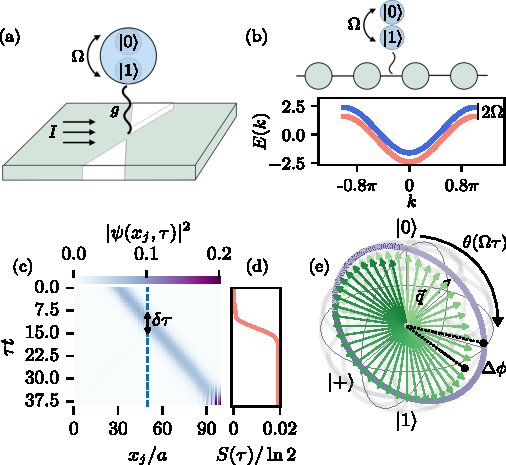
\includegraphics[width=1.0\linewidth]{Figures/fig1.pdf}
    \caption{(a) Schematic of the measurement of a qubit by a QPC. The QPC is a two-dimensional electron gas in the presence of a constriction, through which current $I$ flows due to a voltage bias. The qubit is a double quantum dot with states \mbox{$|0 \ (1)\rangle$} undergoing Rabi oscillations at a frequency \mbox{$\Omega$}, which is capacitively coupled to the QPC current with strength $g$. (b) Schematic of the Hamiltonian Eq.~\eqref{eq:qpc_dd_H} with the eigenenergies Eq.~\eqref{eq:decoupled_energies} of the total system \mbox{$E_{\nu}(k)$}. (c)-(d) Example of a Von Neumann measurement kick for \mbox{$g=0.2$}, \mbox{$k_0 = \pi/3$}, \mbox{$\Omega = 0.1$}. (c) The QPC occupation as a function of time $\tau t$.  the location \mbox{$x_b$} of the bond site as the dashed line. (d) The dynamics of the qubit in the absence of  (blue dots) and presence of  (green arrows) measurement, where darker colors indicate a later points in time. The black arrow represents the qubit's state when the wavepacket arrives at the bond as detailed in Appendix \ref{app:numerical_setup}.}
    \label{fig:fig1}
\end{figure}

\sj{In order to study the dynamics, we first need to specify the initial conditions. When a particle enters the QPC, it will be decoupled from the qubit initially. Hence we work with a product state of the form
\begin{align}\label{eq:initial_state}
    \ket{\Psi(0)} = \ket{\psi}\otimes\big(\cos{\frac{\theta_0}{2}}\ket{0}+\sin{\frac{\theta_0}{2}}e^{i\phi_0}\ket{1}\big).
\end{align}
The state of  the QPC particle \mbox{$|\psi\rangle$}  is a traveling gaussian wavepacket centered around position \mbox{$x_c$}, with an initial group velocity \mbox{$v_g(k_0) = 2 a t\sin(a k_0)$} and width \mbox{$\Delta$}, represented by
\begin{subequations}\label{eq:gauss_wavepacket}
    \begin{align}
    &\ket{\psi} = \sum_{j=1}^N\psi(x_j,x_c,k_0) \hat{c}_j^{\dagger}|\text{vac}\rangle \\
    &\psi(x_j,x_c,k_0) = \left(\frac{1}{\pi \Delta^2}\right)^{1 / 4} e^{-\frac{1}{2 \Delta^2}\left(x_j-x_c\right)^2+i k_0\left(x_j-x_c\right)},
\end{align}
\end{subequations}
where \mbox{$x_j= j a$} denotes the position, and \mbox{$|\text{vac}\rangle$} the vacuum in the QPC. Here we note that although \mbox{$\Delta$} and the wavenumber \mbox{$k_0$} are independent parameters, we are only interested in wavepackets travelling to through the QPC, and as such the wavepackets are composed of eigenmodes with positive momenta. Hence we require \mbox{$1/\Delta<k_0$}.

The qubit is initialized on the Bloch sphere with polar \mbox{$\theta_0$} and azimuthal \mbox{$\phi_0$} angles. In order to calibrate our measurements, we fix the values of \mbox{$\theta_0$} and \mbox{$\phi_0$} such that the qubit is always in the state \mbox{$\frac{1}{\sqrt{2}}(0.9\ket{0} + 0.1\ket{1})$} when the wavepacket is centered on the qubit. We choose this state, as the particle in the QPC will have a finite probability of not interacting with the qubit.
This set of initial conditions implies that the angles are functions of  \mbox{$\omega$} and \mbox{$k_0$}. Appendix~\ref{app:numerical_setup} contains the specific details.}
 
\section{Results}\label{sect:results}

\subsection{Unitary Time Evolution with the Wavepacket}\label{sect:unitary_evolution}

We explicitly solve for the unitary time evolution by performing ED on Eq.~\eqref{eq:qpc_dd_H} for a QPC of \mbox{$N = 100$} sites to obtain the full interacting eigenspectrum. Here we work in dimensionless units where the energies are measured in units of \mbox{$t$} and positions in units of \mbox{$a$}. For the remainder of this work we present results for \mbox{$g = 0.1$} and \mbox{$\Delta = 7$}, unless otherwise specified.

A characteristic example of the dynamics of \mbox{$\ket{\Psi}$} [cf. Eq.~\eqref{eq:initial_state}] is shown in Fig.~\ref{fig:fig1}(c). Here, the center of the wavepacket moves through the QPC according to Ehrenfest's theorem. At a time \mbox{$\tau^* \approx (x_b -x_c)/v_g(k_0)$} the wavepacket is centered on the qubit with a time-evolved width denoted as \mbox{$\Delta(k_0)$}. At this point, the QPC interacts with the qubit for a finite time window. Afterwards, the wavepacket and the qubit evolve independently of one another, undergoing unitary dynamics until the wavepacket is reflected off the end of the chain. In order to avoid such finite size effects, we end our simulations when the center of the wavepacket reaches the last QPC site.

We approximate the measurement time as $\delta \tau = \Delta (k_0)/v_g$, which is the amount of time it takes the wavepacket to completely cross the qubit, according to Ehrenfest's theorem. In this approximation the effective measurement strength is $g\delta \tau$. As $k_0$ approaches its maximum value of $\pi/2$, the wavepacket spreads less and the group velocity increases, thus leading to weaker measurements. Conversely, as $k_0$ approaches \mbox{$1/\Delta \approx k_0$} the trajectories become ill-defined and the semiclassical approximation of the wavepacket breaks down. In this work, we avoid such cases and focus on parameter regimes where there is a well defined measurement time.

\subsection{Measurement Backaction on the Qubit}\label{sect:backaction}

% For vertically stacked fig 2 -----
\iffalse
\begin{figure}
  \centering
    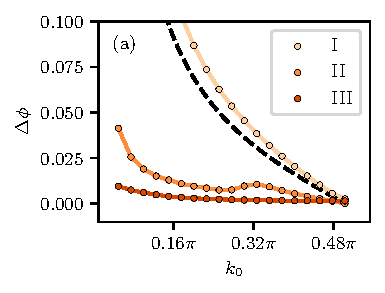
\includegraphics[width=0.75\linewidth]{Figures/phase_v_k0.pdf}
    \\
    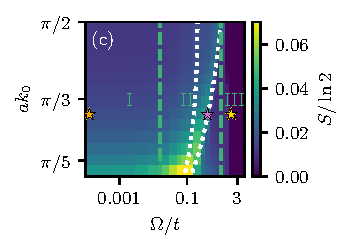
\includegraphics[width=0.75\linewidth]{Figures/entropy_vs_K0_and_om.pdf}%
  \caption{Measurement induced backaction and entanglement on the qubit, with the three observed regimes labeled as I) slow qubit, II) coherent and III) Floquet . (a)-(b) Phase shift and entanglement as a function of \mbox{$k_0$} for three different Rabi frequencies. ED results are shown as red dots and the dashed lines were obtained with Eq.~\eqref{eq:phase_gain} and Eq.~\eqref{eq:dephasing_factor}. (c) Color map for the entropy as a function of \mbox{$k_0$} and \mbox{$\omega$}, the dashed lines  indicate the boundaries between regimes. The points marked with the star symbols correspond to each other in both figures.}\label{fig:fig2}
\end{figure}
\fi

% For horizontal  fig 2 -----
\begin{figure*}
  \centering
    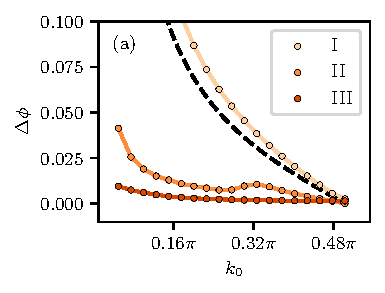
\includegraphics[width=0.32\linewidth]{Figures/phase_v_k0.pdf}
    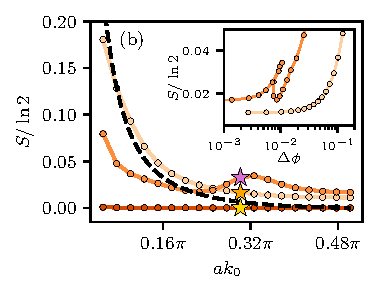
\includegraphics[width=0.32\linewidth]{Figures/entropy_v_k0.pdf}
    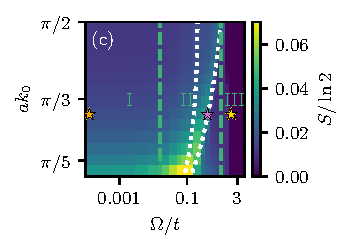
\includegraphics[width=0.345\linewidth]{Figures/entropy_vs_K0_and_om.pdf}
  \caption{Measurement induced backaction and entanglement on the qubit, with the three observed regimes denoted with by roman numeral as slow qubit being I , coherent II and fast qubit III. The von Neumann entropy $S$ is normalized by $1/\ln{2}$. (a)-(b) Phase shift and entanglement as a function of \mbox{$k_0$} for three Rabi frequencies, each representing a regime. For regime I \mbox{$\Omega = 10^{-4}t$}, for regime II \mbox{$\Omega = 0.4t$} and for regime III \mbox{$\Omega = 2.0t$}. ED results are shown as red dots and the dashed lines were obtained with Eq.~\eqref{eq:phase_gain} and Eq.~\eqref{eq:entropy_fit}. (c) Color map for the entropy as a function of \mbox{$k_0$} and \mbox{$\omega$}, the dashed lines  indicate the boundaries between regimes where the boundary between I and II is at \mbox{$\Omega = (1/2) \text{min}[\Delta E (k,p)]$} and the boundary between II and II is at \mbox{$\Omega = t$}. The white dotted line indicates when $k_0$ best fulfills the resonance condition [See Section \ref{sect:entanglement}]. The points marked with star markers correspond to each other in both figures (b) and (c).}\label{fig:fig2}
\end{figure*}

We characterize the effects of measurement in terms of the qubit's Bloch vector \mbox{$\vec{q}$}. An example is shown in Fig.~\ref{fig:fig1}(d), where we compare the qubit's orbits in the presence and absence of the QPC. The dynamics of the qubit are initially identical to free Rabi oscillations, as the particle in the QPC has yet to reach the qubit. When the wavepacket overlaps with the qubit, the interaction leads to entanglement and measurement backaction. 
\sj{At leading order, the backaction manifests as a phase shift $\Delta\phi$, arising because \mbox{$\hat{H}_I$} breaks the quantum non-demolition condition \cite{svensson2013}. At higher orders, the magnitude of the Bloch vector of the qubit \mbox{$\vec{q}$} decreases, as entanglement generated by the measurement leads to the formation of a mixed state in the qubit.}
In addition, one expects at higher orders there is a change in the Rabi frequency \cite{korotkovMeasurementDoubleDot1999, gurvitz1997}. However, we do not observe such a change in our results (see Appendix~\ref{app:derivation_backaction}). After the interaction, the qubit resumes its free Rabi oscillations.

As shown in Fig.~\ref{fig:fig1}(c), the qubit experiences backaction only during the measurement time. Consequently, the incident wavepacket momentum $k_0$, is expected to strongly influence the backaction and entanglement through $g\delta \tau$. To quantify this dependence, Figs.~\ref{fig:fig2}(a) and \ref{fig:fig2}(b) show the phase shift \mbox{$\Delta\phi$} together with the von Neumann entropy, defined as \mbox{$S=\tr{\hat{\rho}_q\log{\hat{\rho}_q}}$}, where \mbox{$\hat{\rho}_q$} is the reduced density matrix of the qubit. Both \mbox{$\Delta\phi$} and \mbox{$S$} are plotted as functions of \mbox{$k_0$} for three Rabi frequencies, \mbox{$\Omega/t=10^{-4},0.4$, and $2.0$}. These frequencies represent three distinct dynamical regimes, characterized by the dimensionless parameter \mbox{$\Omega\delta\tau$}, each exhibiting qualitatively different behavior in both the phase shift and the entanglement entropy.

In the slow qubit regime (\mbox{$\Omega\delta\tau\ll1$}) [corresponding to \mbox{$\Omega/t=10^{-4}$} in Fig.~\ref{fig:fig2}], the qubit remains effectively stationary throughout the interaction with the wavepacket. As a result, the backaction is determined solely by the effective measurement strength. In Figs.~\ref{fig:fig2}(a)-(b), both the phase shift \mbox{$\Delta\phi$} and entanglement entropy \mbox{$S$} from ED decrease monotonically with $k_0$, since \mbox{$\delta\tau$} decreases with increasing $k_0$, due to faster wavepackets. This regime corresponds to \sj{von Neumann non-demolition measurements} \cite{braginskyNondemolition1996} under the assumption \mbox{$\Omega\delta\tau \ll \delta\tau g \ll \delta\tau/t$} [see Appendix~\ref{app:derivation_backaction}], which is consistent with the conditions in \cite{korotkovMeasurementDoubleDot1999, gurvitz1997}. To leading order in \mbox{$g\delta \tau$} we obtain the expression for the phase shift 
\begin{align}\label{eq:phase_gain}
    \Delta \phi (k_0) = \frac{g}{\sqrt{2\pi}t\tan{(ak_0)}} +\mathcal{O}((\delta \tau g)^2), 
\end{align}
 \sj{whereas an expression for von Neumann's entropy \mbox{$S(k_0)$} corresponds to higher order on \mbox{$\Omega \delta \tau$} which break the non-demolition condition} [see Appendix~\ref{app:derivation_backaction} for more details], \sj{and is therefore fitted to an exponential function}. \sj{The analytic} expectation from Eq.~\eqref{eq:phase_gain} \sj{and the exponential fit Eq.\eqref{eq:entropy_fit}} are plotted in Figs.~\ref{fig:fig2}(a)-(b) next of to exact quantities from the numerics.

In the opposite limit is the fast qubit regime (\mbox{$\delta \tau\Omega \gg 1$}) [\mbox{$\Omega/t = 2.0$} in Fig.~\ref{fig:fig2}]. There the phase shift $\Delta \phi$ and entanglement entropy $S$ are approximately zero, independent of $k_0$. This indicates that the QPC and qubit are effectively decoupled from one another due to the mismatched timescales. This can be intuitively understood as the comparatively slow wavepacket only sensing the average qubit's density, which is effectively equivalent to a static potential barrier for the QPC.

Between these limits is  the intermediate coherent regime (\mbox{$\delta \tau \Omega  \approx 1$}) [\mbox{$\Omega/t = 0.4$} in Fig.~\ref{fig:fig2}], which exhibits a pronounced peak in both \mbox{$\Delta\phi$} and \mbox{$S$} at $k_0 \approx 0.3\pi$, in addition to the overall decrease in the phase gain. More strikingly, for $k_0\gtrsim 0.3\pi$, the entropy in the coherent case is larger for slow-qubits, while $\Delta \phi$ is smaller. Such behavior suggests that the measurement efficiency (defined as \mbox{$\Delta \phi / S$}) is enhanced in the coherent regime for suitable values of $k_0$ and $\Omega$.

We can gain more insight into these three regimes and the enhanced measurement efficiency by systematically exploring the entanglement entropy as a function of both \mbox{$k_0$} and \mbox{$\omega$}, as shown in Figure~\ref{fig:fig2}(c). In the slow-qubit regime [I] the entropy is constant in $\Omega$, but becomes larger as $k_0$ decreases, consistent with Fig.~\ref{fig:fig2}(b). In the fast qubit regime [III], the entropy vanishes regardless of $k_0$ and $\Omega$.

Only in the coherent regime [II] do we observe a pronounced peak in the entanglement entropy, confined to a narrow band in the $(\Omega,k_0)$ parameter space. For $k_0$ approaching $\pi/2$, this band is restricted to a narrow range of Rabi frequencies close to $t$. As $k_0$ decreases, however, the region broadens due to the longer measurement times, until the \sj{measurement-kick picture} is no longer valid. Nevertheless, regardless of the values of $k_0$ and $\Omega$, this enhanced entropy band is absent in both the slow [I] and fast qubit [III] regimes, indicating that it is a unique feature of the coherent regime.
 
In the following section, we discuss the physical mechanism behind the enhanced measurement band in Fig.\ref{fig:fig2} and derive quantitative bounds between the three regimes in terms of the Rabi frequency.

\subsection{Inelastic Scattering and Entanglement}\label{sect:entanglement}

\begin{itemize}
    \item  In order to characterize the mechanism behind the resonant band, we calculate the perturbative corrections to the eigenstates of $\hat{H}$, [Appendix \ref{app:derivation_perturbative}].

    \item We obtain Eq.~\eqref{eq:psi_first_order} with three terms, where  Greek indices indicate the band label \mbox{$\pm$}, \mbox{$\bar{\nu} \neq \nu$} always, and \mbox{$\xi(k,p) = \sin{(x_bk)}\sin{(x_b p+p)}+\sin{(x_b p)}\sin{(x_b k+k)}$}.   
\end{itemize}

\begin{widetext}
\begin{equation}
    \ket{\Phi_\nu^{(1)} (k)} = \frac{g\delta\tau}{N+1} \frac{\xi(k,k)}{2\epsilon_\nu} \ket{k} \otimes \ket{\bar{\nu}}+\frac{g\delta\tau}{N+1} \sum_{p \neq k} \ket{p} \otimes \left\{\frac{\xi(k,p)}{-2J(\cos k - \cos p)} \ket{\nu} + \frac{\xi(k,p)}{2\epsilon_\nu - 2J(\cos k - \cos p)} \ket{\bar{\nu}} \right\} \label{eq:psi_first_order}
\end{equation}
\end{widetext}

\begin{itemize}
    \item The first term, has band-mixing and is degenerate when \mbox{$\Omega \rightarrow 0$}, meaning it hybridizes bands and generates entanglement in the slow-qubit regime (I), corresponding to an spontaneous excitation on the qubit \sj{(Not quite sure about this, I am trying to think in terms of diagramatics)}. 

    \item The second term does not mix bands and is only degenerate at the edges of the Brillouin zone. it corresponds to the typical corrections of scattering in tight-binding chain off of a static potential and generates no entanglement between bands.

    \item The third term hybridizes bands and is degenerate when the difference in momentum energy between different bands is equal to the band-gap (resonant condition), corresponding to inelastic scattering that generates an excitation on the qubit.

    \item This resonance condition from the second term can be compared with the exact eigenspectrum in Fig.~\ref{fig:fig3}, where \ref{fig:fig3}(a) plots the exact interacting eigenenergies colored by the projection \mbox{$\Pi_+ = \id_{\text{QPC}}\otimes\ket{+}\bra{+}$} onto the symmetric state, and \ref{fig:fig3}(b) shows the entropy contributions of each eigenstate obtained via the Schmidt decomposition [Appendix \ref{app:numerical_setup}] also colored by band.

    \item In Fig.~\ref{fig:fig3} that the largest entropy peaks correspond to states that fulfill the resonant condition, and also are the most hybridized.

    \item \sj{Secondary entropy peaks correspond to higher order inelastic scattering processes [Appendix \ref{app:derivation_perturbative}]}

     \item This type of inelastic scattering is only possible when $\Omega$  is between the bounds in Eq.~\eqref{eq:entropy_bounds}, that were used to obtain the vertical lines separating the regimes in Fig.~\ref{fig:fig2}(c), in addition the resonant condition is used to obtain the line tracing the enhanced measurement band in the same figure.

\end{itemize}
 
\begin{align}\label{eq:entropy_bounds}
    \frac{1}{2} \text{min}|\Delta E(k,p)| \leq \Omega \leq t  
\end{align}

\begin{figure}
    \centering
    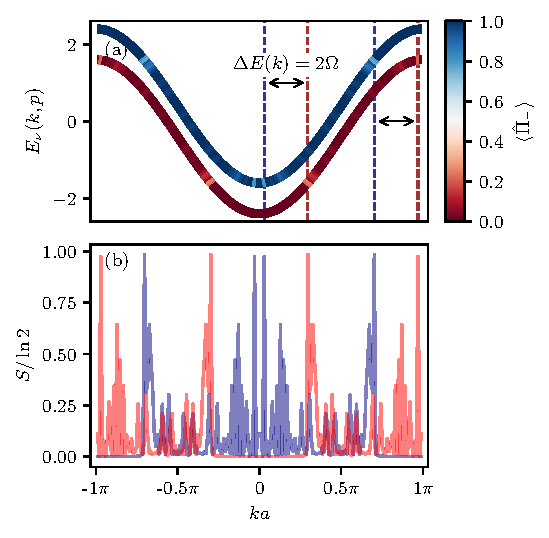
\includegraphics[width=1.0\linewidth]{Figures/band_struct_main.pdf}
    \caption{ED band structure and entanglement for $\omega = 0.4J$ separated into symmetric (Blue), anti-symmetric (red) and labeled by momentum k. (a) Entanglement of each eigenvector of $\hat{H}$. (b) Eigenenergies colored by the projection onto the symmetric band of their respective eigenvectors. The vertical lines indicate the 4 most entangled eigenstates, where dashed/solid lines indicating the resonance.}\label{fig:fig3}
\end{figure}

\section{Discussion and Outlook}\label{sect:disc_outlook}

\begin{itemize}
    \item We proposed a simple Hamiltonian model for the
    QPC-qubit measurement process, with main parameters $k_0$, $\Omega$, that allows us to go beyond the typical current based calculations, and maintain unitary dynamics, thus we find three regimes by looking at the entanglement and backaction. 

     \item The slow qubit regime [I] shows behavior consistent with typical continuous measurement \cite{korotkovSelectiveMeasurement2001, gurvitz1997}, (\sj{Add more papers to this}) which is reflected in the entropy shown in Fig~\ref{fig:fig2}(b) interpreted as an exponential decrease in coherence as a fucntion of the measurement time.
 
    \item The fast qubit regime, shows that the QPC and qubit are decoupled due to a mismatch in their individual timescales.
\end{itemize}

\begin{itemize}
    \item Interestingly, the coherent regime exhibits unique behavior, characterized by a resonant condition between the QPC's kinetic energy and the band-gap between qubit states, that is not possible in Regimes [I] and [III].

     \item When the wavepacket's central momentum $k_0$ fulfills the resonance condition, it predicts the band in Fig~\ref{fig:fig2}(c), indicating that the gaussian weights select which eigenstates dominate at the time of interaction with the qubit. \sj{Make sure to discuss that the white line that corresponds to the peak of the band is also the point where the scattering channel opens up. Check my obsidian notes for this argument}. \sj{(Elaborate here on how this related the time dependent operator picture with the state based one)}.

    \item This inelastic scattering is reminiscent of those found in Fano resonances where the interference between a scattering channel within a continuum and a secondary channel that results in an excitation in a discrete state results in a resonant effect, most clearly observed in a peak (or dip) in transmission \cite{kobayashiFano2004} (Here we need more lit).

    \item In this sense, the resonant line can be traced to the existence of novel many-body effects in QPC's interacting with small systems \cite{ouyangBackaction2010, youngInelasticBackaction2010, snymanPolarization2007} \sj{Here it is important to differentiate and remark that we have a minimal purely unitary model, only using the basic postulates of QM}.

    \item Our results suggest, the the potential of realizing more efficient measurement protocols by relaxing the non-demolition condition, for fast-oscillating qubits, which is necessary to implement quantum gates \cite{wangExperimentalNonadiabatic2016}. 

    \item To further elaborate on the many body connection, our model and methodology can be extended to sequences of wavepackets interacting with the qubit one after the other, which also opens up the possibility of implementing tests for Legget-Garg inequalities \cite{jordan2008}.

    \item In addition, our methodology can be generalized to spin and valley degrees of freedom, relevant to silicon/germanium based quantum dot qubits.

    \item We expect that our results should be seen in experiments when the bias (...).
\end{itemize}

\section{Acknowledgments}

This project was funded by (...)

\section{RDM Statement}


\bibliographystyle{apsrev4-2} % APS recommended BibTeX style
\bibliography{qpc}     % Name of your .bib file (witho

\appendix 

\onecolumngrid 

\section{Numerical Methods and Finite Size Effects}\label{app:numerical_setup}

\subsection{Exact Diagonalization Setup}

\begin{itemize}
    \item Exact diagonalization.
    \item Exact numerical values used.
    \item Initialization of the independent state and estimation of the final state to avoid finite size effects simulation time with ehrenfest.
    \item Estimation of the phase.
    \item Schmidt decomposition.
    \item Mention finite size
\end{itemize}

As mentioned in the main text, we calculate the time evolution of the composite qubit-QPC system, by performing exact diagonalization on the Hamiltonian Eq.~\eqref{eq:qpc_dd_H}. 

The specific form of the free Hamiltonian and the interaction lends itself to exact diagonalization due to the size of its Hilbert space. The model is effectively a one dimensional system restricted to the 2 particle sector of the full Hilbert space, where there is always exactly one excitation on the QPC and one on the double dot. Therefore,  Eq.~\eqref{eq:qpc_dd_H} is expressed as a $2N$ dimensional matrix (where $N$ is the number of QPC lattice sites) in the computational basis
\begin{align}\label{eq:string_basis}
    \ket{\vec{j}}\otimes \ket{\alpha} = \ket{0\dots \overbrace{1}^{j\text{th site}} \dots0}\otimes\ket{\alpha}
\end{align}
where the notation \mbox{$\ket{\vec{j}}$} represents a size $N$ string of zeros with a single one on site $j$. This is the numerical representation of the abstract vectors \mbox{$\hat{c}_j\ket{\text{vac}}$}. The doubling of the matrix's dimension comes from the qubit's states \mbox{$\ket{\alpha} = \ket{0},\ket{1}$}.

The time evolution is performed by computing the exact eigenvectors and values Eq.~\eqref{eq:qpc_dd_H} and applying the time evolution operator
\begin{align}\label{eq:time_evolution_ed}
    \ket{\Psi{(\tau)}} = e^{i\tau/\hbar \hat{H}}\ket{\Psi (0)},
\end{align}
where the initial state \mbox{$\ket{\Psi (0)}$} (Eq.~\eqref{eq:initial_state}) is transformed to the computed eigenbasis. The evolution is carried out until the wavepacket hits the end of the chain, to avoid reflections. The time of flight is given by Ehrenfest's theorem as
\begin{align}\label{eq:final_time}
    \tau_f = \frac{x_N}{v_g} =  \frac{a N}{2 J \sin{k_0a}}
\end{align}
for a semiclassical wavepacket sharply peaked around $k_0$.

Regarding the initial state of the qubit, as mentioned in Section \ref{sect:unitary_evolution}, the initial polar angle $\theta_0$ is dependent on the central wavenumber $k_0$ of the gaussian wavepacket. The reason for this restriction is to guarantee that the qubit is always in the same state when the wavepacket arrives at the bond site and they interact. This allows us to separate the effects of $k_0$ and $\omega$ from those due to a variable qubit occupation. 

Considering a free qubit that passes trough the poles of the Bloch sphere, the initial state is given by the polar angle
\begin{align}\label{eq:qubit_init}
    \theta_0 = - \frac{\theta_b}{2}+\delta\tau \omega
\end{align}
where $\theta_b$ is the free parameter setting the setting the state of the qubit at the time of interaction, and $\Delta \tau$ is the flight time of the wavepacket 
\begin{align}
    \delta \tau = \frac{x_b}{2J\sin(k_0)},
\end{align}
as given by Ehrenfest's theorem.

\sj{The parameters used to create the data presented are \mbox{$N=100$}, \mbox{$a=1$},\mbox{$J=1$}, \mbox{$g=$} \mbox{$k0\in1$}, \mbox{$\omega\in1$}, \mbox{$\theta_f=$}.}



\subsection{Numerical Estimation of Observables}

\begin{align}\label{eq:app_schmidt_deco}
    \Phi = 
\end{align}

\begin{align}\label{eq:entropy_fit}
    S(k_0) = \text{Include the fitting error here}
\end{align}

 \sj{ Include a figure showing how th change in Rabi fremains constant}

 

\section{Von Neumann's Measurement Scheme}\label{app:derivation_backaction}

The following toy model is a realization of von Neumann's measurement kick, appropriate for our Eq.\eqref{eq:qpc_dd_H}. In order to simplify the interaction picture representation of the coupling Hamiltonian Eq.~\eqref{eq:H_int}, we replace the finite lattice with an infinite chain which allows us to write the interaction
in terms of the wavenumber operator $\hat{K}$ as
\begin{align}\label{eq:hint_toy}
    \hat{h}_I = g \hat{K} \otimes \ket{1}\bra{1},
\end{align}
where $\hat{K}$ is defined by its action \sj{(Explain crystal momentum and why it generates a translation in the wavepacket)}
\begin{align}
    \hat{K}\ket{k} = 
\end{align}
and commutes with the infinite tight-binding chain. 

The advantage of this model is that now, the commutator between the free Hamiltonian $\hat{H}_0 =\hat{H}_D + \hat{H}_S$ and the interaction is
\begin{align}
    \left[\hat{h}_I, \hat{H}_0 \right] = -ig\Omega \hat{K}\otimes\hat{\sigma}_y
\end{align}
where we used the fact that \mbox{$\ket{1}\bra{0}+\ket{0}\bra{1}=\hat{\sigma}_x$} and the local density operator is $\ket{1}\bra{1} = \frac{1}{2}(\id -\hat{\sigma}_z)$ in terms of the Pauli matrices. Meaning, when \mbox{$1/\Omega$} is much larger than the measurement time $\delta \tau$, the interaction picture representation is trivial
\begin{align}
    \tilde{h}_I(\delta \tau) = e^{i\delta\tau \hat{H}_0}\hat{h}_I e^{-i\delta\tau \hat{H}_0} = \hat{h}_I
\end{align}
and subsequently the time evolution operator is \mbox{$\tilde{U}(\delta\tau) = \hat{U}(\delta\tau)$} where we donate interaction picture operators with a tilde, instead of a hat. This tells us that, the condition for slow qubit is the same condition for non-demolition measurement (\sj{Cite the new non-demolition papers i found in journal [2026-08-17]}).

We now continue operating under this slow qubit assumption,to calculate the entangled density matrix
\begin{align}
    \tilde{\rho}(\delta\tau)& =  \hat{U}(\delta \tau) \hat{\rho}\hat{U}^{\dagger}(\delta\tau) \nonumber \\ 
    & = e^{-i\delta\tau \hat{h}_I}\ket{\psi (x_b)}\otimes \ket{q}\bra{\psi(x_b)}\otimes\bra{q},
\end{align}
where \mbox{$\ket{\psi(x_b)}$} is Eq.~\eqref{eq:gauss_wavepacket} after enough time has passed that the wavepacket is centered at the bond $x_b$ and \mbox{$\ket{q} = \cos{\theta_b/2}\ket{0}+\sin{\theta_b/2}e^{-i\phi_0}\ket{1}$} is the qubit's state at that point in time. We can easily calculate the action of $\hat{U}$ on the composite system by noticing that $\hat{K}$ is the generator of translations, so it acts as \mbox{$e^{i\lambda \hat{K}}\ket{\psi(x_c)} = \ket{\psi(x_c-\lambda)}$}. The result is 
\begin{align}
    \tilde{\rho}(\delta\tau) & =  \cos^2{\frac{\theta_b}{2}}\ket{\psi(x_b)}\bra{\psi(x_b)}\otimes \ket{0}\bra{0} \nonumber \\ 
    & + \sin^2{\frac{\theta_b}{2}}\ket{\psi(x_b-g\delta\tau)}\bra{\psi(x_b-g\delta\tau)}\otimes\ket{1}\bra{1} \nonumber \\ 
    & + \cos{\frac{\theta_b}{2}}\sin{\frac{\theta_b}{2}}e^{-i\phi_0}\ket{\psi(x_b)}\bra{\psi(x_b-g\delta\tau)}\otimes\ket{0}\bra{1} + \text{h.c}
\end{align}
\sj{what happens to these translations when we have a lattice and it falls in between orbitals?}, where the position of the wavepacket has become coupled to the density at state $\ket{1}$ in the qubit. 

The reduced density matrix is found by taking the partial trace over the QPC degrees of freedom
\begin{align}
    \tilde{\rho}_q(\delta\tau) = \sum_{j}\bra{\vec{j}}\tilde{\rho}(\delta\tau) \ket{\vec{j}}.
\end{align}
The diagonal elements involve sums over the absolute value of the coefficients
\begin{align}
    \sum_j |\psi_j(x_b)|^2 = \sum_j |\psi_j(x_b-g\delta\tau)|^2 = 1
\end{align}
in terms of the coefficients \mbox{$\psi_j(x_b)=\bra{j}\ket{\psi(x_b)}$} as defined in Eq.~\eqref{eq:gauss_wavepacket}. Since these are gaussian coefficients they are normalized to one, and there is no change in the diagonals.

The off-diagonals however, involve the sum of overlaps
\begin{align}
    \sum_j \psi_j(x_b)\psi^{*}_j(x_b-g\delta\tau)  & = \frac{1}{\sqrt{\pi}\Delta} e^{-i g \delta\tau k_0}\sum_{j} \exp{-\frac{(g\delta\tau)^2 + 2(x_b-x_j)^2 - 2 g\delta\tau (x_b-x_j)}{2\Delta^2}},
\end{align}
given that we work in the semi-classical wavepacket limit when \mbox{$\Delta \gg a $}, we approximate the sum as a gaussian integral and obtain 
\begin{align}
\sum_j \psi_j(x_b)\psi^{*}_j(x_b-g\delta\tau) = \exp{-i g\delta\tau k_0  - \frac{3(g\delta\tau)^2}{4 \Delta~2}}.
\end{align}
Here, notices that we are dealing with the wavepacket after it has travelled the distance to $x_b$, so its spread is not the initial \mbox{$\Delta_0$} but \mbox{$\Delta = \Delta_0\sqrt{1+\left(\frac{2\tau_b t \cos{k_0a}}{\Delta_0^2}\right)^2}$},, which is the spread of a Gaussian wavepacket in a lattice. The time of flight to the bond \mbox{$\tau_b  = \delta x/v_g$} is given by Ehrenfest's theorem. Using this expression in the definition for \mbox{$\delta\tau=\Delta/(\sqrt{2}v_g)$} yields the form
\begin{align}
    \sum_j \psi_j(x_b)\psi^{*}_j(x_b-g\delta\tau) = R e^{-i \Delta\phi}
\end{align}
where we define \mbox{$R= e^{\frac{- 3 g^2}{8\sqrt{2}t\sin k_0a}}$} and \mbox{$\Delta \phi = \frac{g\Delta}{2\sqrt{2} t \sin k_0a}$}. So the reduced density matrix in the Bloch sphere is 
\begin{align}
    \tilde{\rho}_q(\delta\tau) = \frac{1}{2}(\id_2+\vec{q}\cdot\vec{\sigma})
\end{align}
with the bloch vector
\begin{align}
    \vec{q} = \begin{pmatrix}
        R \sin(\theta_0) \cos{(\phi_0 +\Delta\phi)}\\
        R\sin(\theta_0) \sin{(\phi_0 +\Delta\phi)}\\
        \cos(\theta_0)
    \end{pmatrix}
\end{align}

\begin{itemize}

    \item Applying $\hat{U}$ to $\ket{\Psi}$ results in an entangled state Eq.\eqref{eq:entangled_state} where $\hat{O}$ is correlated with the occupation in the qubit. 
    
    \item Tracing away the QPC degrees of freedom, yields the post measurement qubit density matrix $\hat{\rho}^\prime$ in terms of the Bloch vector in Eq.\eqref{eq:new_q}, with the phase shift $\Delta \phi$ in Eq.\eqref{eq:phase_gain}.

    \item Fitting of the Entropy.
\end{itemize}

\section{Derivation of the Perturbative Corrections}\label{app:derivation_perturbative}
In this appendix we examine the eigenenergies and eigenstates of the total Hamiltonian in Eq.~\eqref{eq:qpc_dd_H} describing the coupled QPC and detector system. We treat \mbox{$g$} as our perturbative parameter, and expand the wavefunction to first order
\begin{equation}
    \ket{\Phi_{\nu} (k)} = \ket{\Phi^{(0)}_\nu (k)} + \ket{\Psi^{(1)}_\nu (k)} +O\left((g/J)^2\right).
\end{equation}
At zeroth order, the eigenstates are labeled by the momentum \mbox{$k$} and the index \mbox{$\nu = \pm$}. The eigenstates are a direct product of the standing waves for the QPC and the symmetric/anti-symmetric qubit states.
\begin{align}\label{eq:app_zero_eigenstate}
    \ket{\Phi^{(0}_\nu(k)} = & \ket{k}\otimes\ket{\nu} =  \sqrt{\frac{2}{N+1}} \sum_{l=1}^{N} \sin{(a kl)} \hat{c}_l\ket{\text{vac}}\otimes \frac{1}{\sqrt{2}}\left(\ket{0} \pm e^{i\phi}\right).
\end{align}

The first order correction to the wavefunction is given by
\begin{align}\label{eq:app_first_order1}
     \ket{\Phi_\nu^{(1)} (k)} = \sum_{(\mu,p)\neq(\nu,k)} \frac{\bra{\phi^{(0)}_\mu (p)}H_1 \ket{\phi^{(0)}_\nu (k)}}{ E_{\nu}^{(0)}(k) -  E_{\mu}^{(0)}(p)} \ket{p}\otimes \ket{\mu}.
\end{align}
The matrix element in the numerator only involves the bond sites
\begin{align*}
    \bra{\Phi^{(0)}_\mu (p)}H_1 \ket{\Phi^{(0)}_\nu (k)} & = g \hat{d}_1^{\dagger}\hat{d}_1\ket{\nu} \bra{p} \hat{c}_{b+1}^{\dagger}\hat{c}_b + \hat{c}_b^{\dagger}\hat{c}_{b+1} \ket{k},
 \end{align*}
 where the inner products are resolved by expressing $\ket{k}$ and $\ket{\nu}$ in the spatial/computational basis Eq.~\eqref{eq:app_zero_eigenstate} and resolving the orthogonality conditions. The result is the expression
 \begin{align}\label{eq:app_matrix_element}
     \bra{\Phi^{(0)}_\mu (p)}H_1 \ket{\Phi^{(0)}_\nu (k)} = \frac{g\xi(k,p)}{N+1} = \frac{g}{N+1} \left(  \sin(abk+ak )\sin(abp)  + \sin(abp+ap)\sin(abk)\right),
 \end{align}
with $b$ indicating the the position of the bond $x_b = ab$, 

\begin{figure}
    \centering
    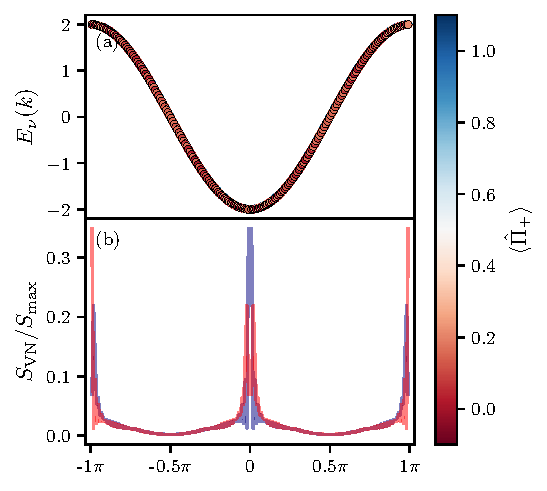
\includegraphics[width=0.45\linewidth]{Figures/band_struct_app_0.001.pdf}
    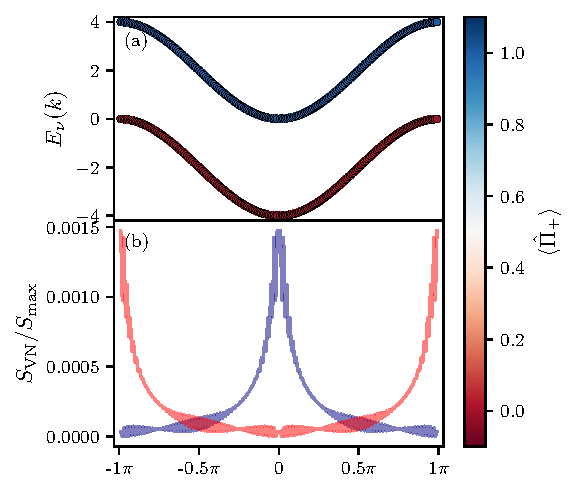
\includegraphics[width=0.45\linewidth]{Figures/band_struct_app_2.000.pdf}
    \caption{(a) ED band structure and entanglement for (a) a slow qubit with \mbox{$\omega = 0.001J$} and (b) a FLoquet qubit \mbox{$\omega = 2.0J$}. The coloring follows the same convention as Fig.~\ref{fig:fig2}, according to the projection onto the symmetric band of their respective eigenvectors, with blue being symmetric and red anti-symmetric.}\label{fig:app_band_structure}
\end{figure}

Having calculated the numerator, it is useful to separate Eq.~\eqref{eq:app_first_order1} into three terms that show when the expansion is degenerate: The first term corresponds to \mbox{$\mu \neq \nu, p=k$}, the second \mbox{$\mu = \nu, p\neq k$} and the third \mbox{$\mu \neq \nu, p\neq k$}. This results in the following form
\begin{equation}
    \ket{\Phi_\nu^{(1)} (k)} = \frac{g}{N+1} \frac{\xi(k,k)}{2\epsilon_\nu} \ket{k} \otimes \ket{\bar{\nu}}+\frac{g}{N+1} \sum_{p \neq k} \ket{p} \otimes \left\{\frac{\xi(k,p)}{-2J(\cos ak - \cos ap)} \ket{\nu} + \frac{\xi(k,p)}{2\epsilon_\nu - 2J(\cos ak - \cos ap)} \ket{\bar{\nu}} \right\} \label{eq:app_first_order2},
\end{equation}
where the bar notation indicates $\bar{\nu}\neq \nu$ explicitly, as also shown in the main text. Each of these terms dominates the eigenstates contributions whenever they become degenerate and, if there is mixing between the symmetric and antisymmetric bands (In our notation these are terms with factors of $\ket{\bar{\nu}}$), they also indicate when the eigenstates become highly entangled according to their Schmidt decomposition Eq.~\eqref{eq:app_schmidt_deco}.

The first term is degenerate when \mbox{$\epsilon_\nu=\pm \omega\rightarrow0$} and involves $\ket{\bar{\nu}}$, therefore it does mix between two different bands but only for slow qubits. For a Hamiltonian in which this term dominates, the entanglement of the eigenstates is compared with the hybridization at each eigenenergy in Fig.~\ref{fig:app_band_structure}(a). The states remain weakly hybridized throughout the spectrum, except for pronounced fluctuations near the maxima and minima of the Brillouin zone. This term dominates in regime [I] as discussed in Section \ref{sect:entanglement}.

On the other hand, the second term is degenerate only in at the edges of the Brillouin zone \mbox{$a k\approx \pm \pi$} but it does not mix between bands, hence it does not contribute to entanglement. This degeneracy is typical for tight-binding Hamiltonians and corresponds to elastic scattering between QPC states. An example of the entanglement and hybridization for a system in which this term dominates is shown in Fig.~\ref{fig:app_band_structure}(b). Here, it is clear that both bands are fully symmetric or antisymmetric and the resulting entanglement entropy of the eigenstates is negligible.

Finally, the third term does mix between bands and becomes degenerate, depending on the whenever the difference in the energy of \mbox{$k$} modes \mbox{$\Delta E (k,p)$} is equal to the band-gap \mbox{$2\epsilon_\nu$}. Since, we consider a finite lattice, \mbox{$\Delta E (k,p)$} is finite, hence a small enough $2 \epsilon_\nu$ (slow qubit) can avoid this degeneracy. Furthermore, a large enough band gap (fast qubit) will always be larger than \mbox{$\Delta E (k,p)$} due the cosine form of the tight-binding energy. These conditions bound the degenerate region as indicated in Eq.~\eqref{eq:entropy_bounds} and dominates the coherent regime [II] as discussed in \ref{sect:entanglement}. This third term can be interpreted in terms of inelastic scattering, where the QPC exchanges momentum energy with the qubit's own eigenenergy .

As mentioned in the main text, the gaussian weights select which of the eigenstates dominate at any given point which gives and interpretation of the eigenstate peaks at the minima/maxima of the Brillouin zone in Fig~\ref{fig:app_band_structure}. The semi-classical approximation of the gaussian wavepacket, necessitate that the weights are sharply peaked around the central wavenumber $k_0$, with a group velocity $v_g = 2 J \sin{(ak_0)}$. The weights then select the largest contribution to the state to be the one with $k \approx k_0$, which in turn can be assigned a group velocity $v_g$. Therefore, the entropy peaks seen in Fig~\ref{fig:app_band_structure} corresponds with $v_g \approx 0$. Following the analysis in Section \ref{sect:backaction}, these states have an ill-defined measurement time window and the QPC and qubit remain coupled. 

\twocolumngrid

\end{document}

